\thispagestyle{fancy}

\begin{center}
  {\LARGE\bfseries Message from the Head\par}
\end{center}

\vspace{0.7cm}
\noindent
\begin{minipage}[c]{0.23\textwidth}
  \centering
  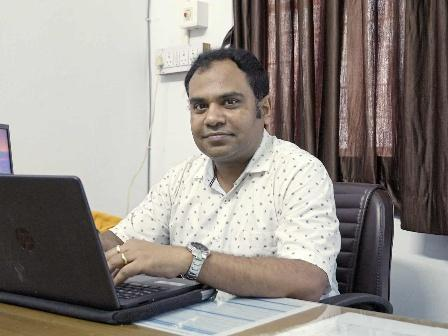
\includegraphics[width=\linewidth]{assets/images/head_prasun_chowdhury.jpg}
\end{minipage}
\hfill
\begin{minipage}[c]{0.72\textwidth}
  {\large\bfseries Dr. Prasun Chowdhury\par}
  \smallskip
  {\itshape Associate Professor \& Head\par}
\end{minipage}

\vspace{0.7cm}
{\justifying
I am delighted to present Volume X of our Departmental Technical Magazine, \textit{Electronic Trends}, a platform that continues to capture the academic excellence, technical curiosity, and creative strengths of our students and faculty members. This edition reflects the steady progress of the department and our commitment to fostering a dynamic learning environment rooted in innovation, research, and collaborative growth.

\medskip
Over the past year, our department has achieved significant milestones---through student projects, research publications, technical workshops, industry interactions, and various academic initiatives that have enriched the overall learning experience. The contributions featured in this volume highlight the dedication, capability, and perseverance of our academic community.

\medskip
This magazine is more than a collection of technical articles; it is a celebration of ideas, exploration, and continuous development. I sincerely appreciate the efforts of the editorial board, faculty coordinators, and student volunteers who have worked diligently to bring out this edition with professionalism and excellence.

\medskip
I encourage all students to actively participate in technical endeavours, stay updated with emerging technologies, and develop the skills necessary to thrive in a rapidly evolving global environment. I am confident that this publication will inspire many to think innovatively, pursue research with passion, and strive for excellence in all their pursuits.

\medskip
My best wishes to everyone involved in making Volume X a meaningful and successful publication.\par}

\medskip
\begin{flushright}
  \textbf{Dr. Prasun Chowdhury}\par
  Associate Professor \& Head\par
  Electronics \& Communication Engineering\par
  {\small St. Thomas' College of Engineering \& Technology, Kolkata\par}
\end{flushright}

\vfill\null